\documentclass[11pt,a4paper]{article}

% ---------- Page setup ----------
\usepackage[a4paper,top=2.3cm,bottom=2.3cm,left=2.2cm,right=2.2cm,headheight=14pt]{geometry}
\usepackage{lmodern}
\usepackage[T1]{fontenc}
\usepackage{microtype}
\usepackage{amsmath,amssymb}
\usepackage[table]{xcolor}
\usepackage[most]{tcolorbox}
\usepackage{fancyhdr}
\usepackage{lastpage}
\usepackage{titlesec}
\usepackage[hang]{footmisc}
\usepackage{enumitem}
\usepackage{booktabs}
\usepackage{tabularx}
\usepackage{xltabular}
\usepackage{array}

\usepackage{tikz}
\usetikzlibrary{positioning,calc,arrows.meta}
\usepackage[colorlinks=true,linkcolor=accent,citecolor=accent,urlcolor=accent]{hyperref}

% ---------- Colours ----------
\definecolor{navy}{HTML}{1F3B5C}
\definecolor{accent}{HTML}{2D6A9F}
\definecolor{boxfill}{HTML}{F3F7FB}
\definecolor{softgray}{HTML}{6B7280}

% ---------- Footnotes ----------
% clear gap above the notes, a full-width accent rule, and wrapped lines aligned after the number
\setlength{\skip\footins}{18pt plus 4pt minus 2pt}
\setlength{\footnotesep}{10pt}
\setlength{\footnotemargin}{1.4em}
\renewcommand{\footnoterule}{\kern-3pt\begingroup\color{accent!45}\hrule width\textwidth height 0.6pt\endgroup\kern2.4pt}

% ---------- Headings ----------
\titleformat{\section}{\Large\bfseries\color{navy}}{}{0pt}{}
\titlespacing*{\section}{0pt}{11pt}{5pt}
\titleformat{\subsection}{\large\bfseries\color{accent}}{}{0pt}{}
\titlespacing*{\subsection}{0pt}{8pt}{3pt}

% ---------- Header and footer ----------
\pagestyle{fancy}
\fancyhf{}
\fancyhead[L]{\small\color{accent}Machine Learning Project Proposal}
\fancyhead[R]{\small\color{accent}FX Returns and Volatility}
\fancyfoot[C]{\small\color{softgray}Page \thepage\ of \pageref{LastPage}}
\renewcommand{\headrulewidth}{0.4pt}

% ---------- Lists and tables ----------
\setlist{itemsep=1pt,topsep=3pt,parsep=0pt}
\newcolumntype{Y}{>{\raggedright\arraybackslash}X}
\renewcommand{\arraystretch}{1.25}
% long tables may break across pages; the header row repeats
\setlength{\LTpre}{4pt}
\setlength{\LTpost}{2pt}
\setlength{\emergencystretch}{3em}
% no automatic hyphenation at line ends
\hyphenpenalty=10000
\exhyphenpenalty=10000
\setlength{\parindent}{0pt}
\setlength{\parskip}{4pt}
% never split a footnote across pages
\interfootnotelinepenalty=10000

\begin{document}

% =====================================================================
%  Title box
% =====================================================================
\begin{tcolorbox}[enhanced,colback=boxfill,colframe=navy,arc=3mm,boxrule=0.8pt,
                  left=5mm,right=5mm,top=4mm,bottom=4mm]
{\LARGE\bfseries\color{navy}Predictability in Currency Markets: Regime-Aware Learning of Returns and Volatility}\\[4pt]
{\large\color{softgray}Project Proposal for the Machine Learning Course (BITS F464)}\\[3pt]
{\itshape\small A walk-forward machine learning study of what is predictable in foreign exchange markets, when it is predictable and whether that predictability has economic value.}

\vspace{5mm}
\begin{center}
{\large\bfseries Group Members}\\[4pt]
SARTHAK SHAH~~(2023AAPS1051G)\\
JASKARAN SINGH~~(2023B5A70959G)\\
ADITYA BHANSALI~~(2023A3PS0187G)\\
R.V. PRADYUMN~~(2023B5AD0973G)\\
PARIKSHITH MOLEYAR~~(2023B1A70654G)\\
M ARUN PRAKASH~~(2024A1PS0305G)\\[8pt]
{\bfseries Date: 29th October 2026}
\end{center}

\begin{tcolorbox}[colback=white,colframe=gray!30,arc=2mm,boxrule=0.4pt,left=4mm,right=4mm,top=2mm,bottom=2mm]
\textbf{Proposal Summary.} Daily exchange rate returns are famously close to a random walk, yet their
volatility is strongly persistent and markets switch between calm and turbulent \emph{regimes}. Rather than
only asking whether tomorrow's price can be predicted, this project measures \emph{which} aspects of currency
markets are predictable, by \emph{which} learning algorithms and \emph{in which} regimes. We build a pipeline free of look-ahead bias over twenty years of minute by minute data for the seven major USD currency pairs, discover
market regimes with unsupervised learning, compare statistical, classical, ensemble and neural models for
volatility and return forecasting under walk-forward validation and backtest the resulting signals against
standard strategies after transaction costs.
\end{tcolorbox}
\end{tcolorbox}

% ---------- At a glance ----------
\begin{tcolorbox}[colback=white,colframe=accent!40,arc=2mm,boxrule=0.5pt,left=1mm,right=1mm,top=1.5mm,bottom=1.5mm]
\centering
\begin{tabularx}{\linewidth}{*{3}{>{\centering\arraybackslash}X}}
{\Large\bfseries\color{navy}7}              & {\Large\bfseries\color{navy}2006--2026}      & {\Large\bfseries\color{navy}$\approx$55M} \\[-2pt]
{\footnotesize\color{softgray}major USD currency pairs} & {\footnotesize\color{softgray}over 20 years of market data} & {\footnotesize\color{softgray}minute price bars} \\
\end{tabularx}
\end{tcolorbox}

% =====================================================================
\section*{Problem Motivation and Background}
% =====================================================================
The foreign exchange (FX) market is the largest financial market in the world with about \$9.6 trillion traded every day. Exchange rates set the cost of international
trade, the value of foreign investments and the risk carried by every institution with currency exposure.
Forecasting them is valuable but notoriously hard: study after study has found that a simple random walk is very difficult to beat when predicting exchange rate changes out of
sample.

Yet the difficulty is not uniform. Daily FX returns are close to unpredictable, but their
\emph{volatility} is strongly persistent: calm days follow calm days and turbulent days cluster
together. Markets also move between distinct \emph{regimes}: quiet trending
periods, crises and sudden shocks such as the Swiss National Bank's removal of the EUR/CHF\footnote{Currency codes: USD US dollar, EUR euro, GBP British pound, JPY Japanese yen, CHF Swiss franc, AUD Australian dollar, CAD Canadian dollar, NZD New Zealand dollar and INR Indian rupee. A pair such as EUR/CHF is the price of one euro in Swiss francs.} floor in
January 2015, the Brexit referendum in 2016, the COVID-19 crash of March 2020 and the unwinding of the yen
carry trade in August 2024. A model that works in one regime may fail badly in another.

Many machine learning studies of financial forecasting also report directional accuracies that vanish under careful evaluation because of \emph{look-ahead bias}: scaling with statistics from the full sample, shuffling time series data during cross-validation or computing features with information from the future. A credible
project must therefore be as careful about \emph{how} models are evaluated as about \emph{which} models are used.

Our project asks a sharper question than ``can we predict tomorrow's exchange rate?'': which aspects of currency markets are predictable, by which class of learning algorithm and in which market regimes? And does any statistical predictability survive transaction costs as genuine economic value?

% =====================================================================
\section*{Project Objectives}
% =====================================================================
The project aims to:
\begin{itemize}
  \item build a data pipeline free of look-ahead bias that turns twenty years of minute by minute quotes for seven currency pairs into daily features and realized volatility targets
  \item discover market regimes with unsupervised learning and validate them against documented market episodes
  \item forecast next day volatility and returns with a broad family of models from linear and probabilistic baselines to ensembles and recurrent neural networks
  \item evaluate every model under a strict walk-forward protocol with statistical significance tests
  \item backtest the models' trading signals and risk forecasts against standard baseline strategies across regimes and stress periods
\end{itemize}
This project satisfies the course requirement of being \textbf{nontrivial} because it combines substantial data engineering (about 55 million intraday observations), four distinct learning tasks (clustering, two
regression problems and a classification problem), a broad range of model families (from linear and probabilistic models to ensembles and neural networks) and an evaluation protocol designed specifically to rule out the look-ahead bias common in
financial machine learning.

% =====================================================================
\section*{Research Questions and Hypotheses}
% =====================================================================
The questions below define the project. The hypotheses are our starting expectations: the project succeeds
whether each one is confirmed or rejected as long as the answer is backed by careful evidence.

{\small
\begin{xltabular}{\linewidth}{>{\bfseries\color{navy}}l Y Y}
\toprule
 & \textbf{Research question} & \textbf{Starting hypothesis} \\
\midrule
\endhead
RQ1 & How much of next day realized volatility can be predicted and do machine learning models improve on econometric benchmarks (GARCH,\footnote{Generalized Autoregressive Conditional Heteroskedasticity: a classic model of time varying volatility.} HAR-RV\footnote{Heterogeneous Autoregressive model of Realized Volatility.})?
    & \textbf{H1.} Volatility is substantially predictable; nonlinear models can match or improve on HAR-RV especially in high volatility regimes. \\
RQ2 & Is the direction of next day returns predictable beyond chance once look-ahead bias is removed?
    & \textbf{H2.} Directional accuracy stays close to 50\% and any statistically significant edge is
      concentrated in specific regimes. \\
RQ3 & Do unsupervised methods recover economically meaningful regimes and do regime-aware models outperform
      a single global model?
    & \textbf{H3.} Regimes align with known crisis episodes and regime-aware models beat global models
      mainly in high volatility regimes. \\
RQ4 & Do statistical forecast gains survive transaction costs and lead to better returns per unit of risk and more reliable risk estimates?
    & \textbf{H4.} Most backtest improvement comes from sizing positions with volatility forecasts rather than from directional calls. \\
RQ5 & How does a generative classifier compare with a discriminative one as the amount of training data changes?
    & \textbf{H5.} Gaussian Naive Bayes is competitive with logistic regression on short training windows while logistic regression wins on long ones. \\
\bottomrule
\end{xltabular}}

% =====================================================================
\section*{Dataset and Inputs}
% =====================================================================
All data used in this project is publicly and \textbf{freely} available: no paid API, subscription or API key
is required. Each source below was checked for free access before writing this proposal.

{\small
\begin{xltabular}{\linewidth}{>{\raggedright\arraybackslash}p{4.0cm} >{\raggedright\arraybackslash}p{3.0cm} >{\raggedright\arraybackslash}p{2.7cm} Y}
\toprule
\textbf{Data} & \textbf{Source} & \textbf{Frequency / span} & \textbf{Role in the project} \\
\midrule
\endhead
Minute bid OHLC\footnote{Open, High, Low and Close: the first, highest, lowest and last price within each bar.} bars for the 7 major pairs & \href{https://www.histdata.com}{HistData.com} (free yearly files) & 1 minute, 2006--2026 & Realized volatility, daily bars, intraday features \\
Gold, crude oil, S\&P 500 & \href{https://www.histdata.com}{HistData.com} & 1 minute & Risk context from other markets \\
VIX,\footnote{Volatility Index: the market's expectation of US stock market volatility over the next 30 days.} nominal broad USD index, H.10\footnote{The Federal Reserve's statistical release of daily foreign exchange rates.} reference rates & \href{https://fred.stlouisfed.org}{FRED},\footnote{Federal Reserve Economic Data: the free public database of the Federal Reserve Bank of St. Louis.} St.\ Louis Fed (CSV, no key) & Daily & Risk sentiment, dollar factor, data checks \\
Central bank policy rates of the 8 currencies & \href{https://data.bis.org/topics/CBPOL}{BIS}\footnote{Bank for International Settlements: an international body of central banks that publishes global financial statistics.} policy rate statistics & Daily & Interest rate differentials (carry) \\
Backup intraday quotes & Dukascopy (via \texttt{dukascopy-node}) & Tick / 1 minute & Gap filling and data checks \\
\bottomrule
\end{xltabular}}

We study the seven most traded USD pairs (\mbox{EUR/USD}, \mbox{GBP/USD}, \mbox{USD/JPY}, \mbox{USD/CHF},
\mbox{AUD/USD}, \mbox{USD/CAD} and \mbox{NZD/USD}) from January 2006 to October 2026. This is the longest window covered by every source. The data amounts to roughly \textbf{55 million minute bars} ($\approx$3\,GB raw) that are aggregated into about \textbf{38,000 daily observations} across the pairs. Each observation is described by a few dozen engineered features. The window contains the 2008 financial crisis, the euro area debt crisis, the 2015 franc shock,
Brexit, COVID-19, the 2022 tightening cycle and the 2024 carry unwind. These episodes serve as natural stress tests.

% =====================================================================
\section*{Proposed Methodology}
% =====================================================================
The workflow has five stages that all sit inside a single walk-forward validation framework. The models named
in each stage are \emph{candidates} rather than a fixed checklist: we start with simple baselines, add models in order of expected value and drop any that prove impractical or add nothing.

\begin{center}
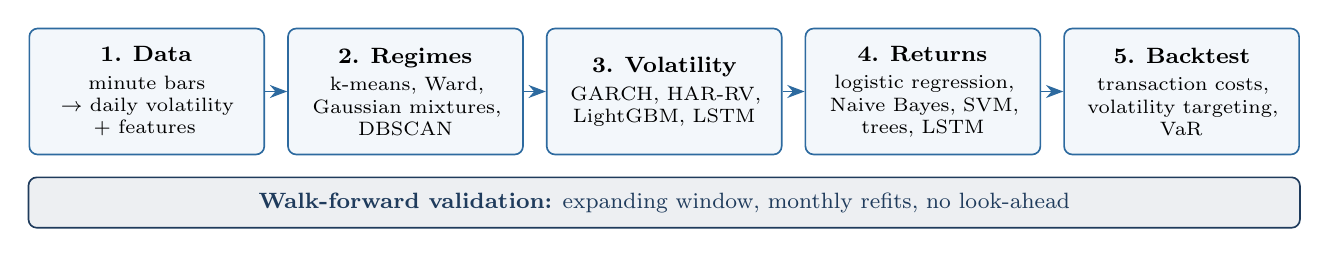
\begin{tikzpicture}[
  stage/.style={draw=accent,fill=boxfill,rounded corners=3pt,line width=0.6pt,
                minimum height=1.6cm,text width=2.75cm,align=center,font=\scriptsize},
  arr/.style={-{Stealth[length=2.2mm]},line width=0.7pt,draw=accent}]
\node[stage] (s1) {{\footnotesize\bfseries 1. Data}\\[2pt] minute bars\\ $\to$ daily volatility\\ + features};
\node[stage,right=0.28cm of s1] (s2) {{\footnotesize\bfseries 2. Regimes}\\[2pt] k-means, Ward,\\ Gaussian mixtures,\\ DBSCAN};
\node[stage,right=0.28cm of s2] (s3) {{\footnotesize\bfseries 3. Volatility}\\[2pt] GARCH, HAR-RV,\\ LightGBM, LSTM};
\node[stage,right=0.28cm of s3] (s4) {{\footnotesize\bfseries 4. Returns}\\[2pt] logistic regression,\\ Naive Bayes, SVM,\\ trees, LSTM};
\node[stage,right=0.28cm of s4] (s5) {{\footnotesize\bfseries 5. Backtest}\\[2pt] transaction costs,\\ volatility targeting,\\ VaR};
\draw[arr] (s1) -- (s2);
\draw[arr] (s2) -- (s3);
\draw[arr] (s3) -- (s4);
\draw[arr] (s4) -- (s5);
\draw[draw=navy,fill=navy!8,rounded corners=3pt,line width=0.6pt]
  ($(s1.south west)+(0,-0.28)$) rectangle ($(s5.south east)+(0,-0.92)$);
\node[font=\footnotesize\color{navy}] at ($(s1.south west)!0.5!(s5.south east)+(0,-0.6)$)
  {\textbf{Walk-forward validation:} expanding window, monthly refits, no look-ahead};
\end{tikzpicture}
\end{center}

\subsection*{1. Data Engineering and Feature Construction}
Raw minute bars are cleaned (duplicate and stale quotes removed and gaps flagged) and aggregated into daily
open, high, low and close prices. The main volatility target is daily \emph{realized variance} computed from intraday five minute returns.
On top of these we will compute features from the groups below; the exact set will be refined during
exploratory analysis:
\begin{itemize}
  \item \textbf{Returns and momentum:} lagged log returns (1--21 days), 1--12 month momentum, distance from moving averages.
  \item \textbf{Technical indicators:} RSI, MACD, Bollinger \%B, ATR, stochastic oscillator, ADX.\footnote{RSI: Relative Strength Index. MACD: Moving Average Convergence Divergence. ATR: Average True Range. ADX: Average Directional Index. \%B: where the price sits within its Bollinger bands.}
  \item \textbf{Volatility:} realized volatility at daily, weekly and monthly horizons, the Parkinson and Garman--Klass range estimators, realized semivariances and GARCH conditional variance.
  \item \textbf{Currency factors:} principal components of the returns of all seven pairs (a ``dollar'' factor and a carry factor) and average pairwise correlation.
  \item \textbf{Macro and risk:} VIX, broad dollar index, policy rate differentials, gold, oil and S\&P 500 returns.
  \item \textbf{Calendar:} day of week and end of month effects.
\end{itemize}
Every feature uses only information available at the close of the day it describes. Every transformation with
fitted parameters (scalers, PCA, GARCH, clustering) is fitted again inside each training window so that no information from the test period can leak into training.

\subsection*{2. Unsupervised Regime Discovery}
Each day is described by a regime vector of realized volatility over short and long horizons, trend strength, correlation across pairs and VIX. We compare four clustering approaches: \textbf{k-means} (hard assignments),
\textbf{agglomerative hierarchical clustering} with Ward linkage (the dendrogram guides the number of regimes),
\textbf{Gaussian mixture models fitted by EM} (soft probabilistic assignments) and \textbf{DBSCAN} (which isolates shock days as noise points). The number of regimes is chosen with the silhouette score, the Davies--Bouldin index and BIC. Regimes are validated by their persistence and by how well they align with
documented episodes. They are then used in two ways: as input features (posterior regime probabilities) and
to train a separate expert model for each regime.

\subsection*{3. Volatility Forecasting (Regression)}
The target is next day log realized volatility. Candidate models fall into three groups:
\begin{itemize}
  \item \textbf{Econometric benchmarks:} the naive forecast (today's volatility), the EWMA\footnote{Exponentially Weighted Moving Average. RiskMetrics is its standard industry version.} (RiskMetrics) model and the GARCH(1,1) and GJR-GARCH\footnote{A GARCH variant in which falls raise volatility more than rises of the same size.} models with Student-$t$ errors estimated by \emph{maximum likelihood}.
  \item \textbf{HAR-RV} is a linear regression on daily, weekly and monthly volatility.
  \item \textbf{Machine learning models} that use the full feature set: ridge and lasso regression, $k$-nearest
        neighbour regression, random forest, LightGBM, a multilayer perceptron and an LSTM over a window of recent days.
\end{itemize}

\subsection*{4. Return Forecasting (Classification and Regression)}
\textbf{Direction.} The classification target is whether the next day return is positive. Candidate models
include logistic regression, Gaussian Naive Bayes, $k$-nearest neighbours, a decision tree, support vector machines (SVM) with linear and RBF kernels, random forest, LightGBM, a multilayer perceptron and an LSTM. All classifiers output probabilities that are also checked for calibration.

\textbf{Magnitude.} The regression target is the next day return itself. Baselines are the random walk (zero) forecast, the historical mean and ARIMA;\footnote{AutoRegressive Integrated Moving Average: a classic linear time series model.} these are compared with regularised linear regression, gradient boosting and a
recurrent network.

Models are trained in both a \emph{global} and a \emph{regime-aware} form wherever regimes prove useful so that the value of regime information can be measured directly. For H5 we also trace learning curves of Naive Bayes against logistic
regression as the training window grows from a few months to many years.

\subsection*{5. Backtesting and Risk Evaluation}
Model signals are compared against simple baselines such as always being long, \emph{carry} (long the currency with the higher interest rate), time series momentum and no trading (the random walk). Strategies driven by the models will include (i) the predicted direction with a confidence threshold, (ii) the same signal with \emph{volatility targeting} (smaller positions when forecast volatility is high) and (iii) a portfolio across all seven pairs with equal risk in each. Realistic bid--ask spreads are charged on every trade and results are checked for sensitivity to higher costs. Volatility forecasts are also turned into daily 99\% Value at Risk (VaR) estimates. All results are broken down by regime, stress period, currency pair and subperiod.

% =====================================================================
\section*{Validation Protocol and Evaluation Metrics}
% =====================================================================
We use a \textbf{walk-forward} design with an expanding window: every model is trained only on data that precedes its test period and is then rolled forward and retrained at regular intervals (monthly as a starting point and less often for slower models such as neural networks). The first several years of data (including the 2008 crisis) form the initial training window. This leaves more than a decade for out-of-sample testing.
Hyperparameters are tuned on the most recent part of each training window with a short embargo gap in between. Data is never shuffled. These rules stay fixed whichever models are finally used because they are what make the results trustworthy. Interpretability will come from tools such as SHAP\footnote{SHapley Additive exPlanations: splits each prediction into contributions from the input features.} values for tree ensembles, permutation importance and model coefficients.

{\small
\begin{xltabular}{\linewidth}{>{\raggedright\arraybackslash}p{2.9cm} >{\raggedright\arraybackslash}p{2.2cm} Y >{\raggedright\arraybackslash}p{4.0cm}}
\toprule
\textbf{Task} & \textbf{Type} & \textbf{Metrics} & \textbf{Significance test} \\
\midrule
\endhead
Regime discovery    & Clustering     & Silhouette, Davies--Bouldin, BIC, alignment with known episodes & -- \\*
Volatility forecast & Regression     & RMSE, MAE, QLIKE,\footnote{Quasi likelihood loss: the standard loss for comparing volatility forecasts.} Mincer--Zarnowitz $R^2$     & Diebold--Mariano \\*
Return direction    & Classification & Accuracy, balanced accuracy, ROC-AUC, Brier score               & Pesaran--Timmermann \\*
Return magnitude    & Regression     & RMSE, MAE, out-of-sample $R^2$ against the zero forecast & Diebold--Mariano \\*
Trading and risk    & Backtest       & Annualised return, Sharpe, Sortino, maximum drawdown, turnover, VaR exceedances & Kupiec \\*
\bottomrule
\end{xltabular}}

% =====================================================================
\section*{Project Scope}
% =====================================================================
The plan is layered so that the project still produces a complete result if some parts prove harder than
expected. We commit firmly to the research questions, the data and the evaluation protocol; the exact model
set, features and parameters will be refined as results come in.
\begin{itemize}
  \item \textbf{Core:} the data pipeline; regime discovery; volatility and return forecasting against baselines and a representative set of learning models; walk-forward evaluation with
        significance tests; and a backtest after transaction costs.
  \item \textbf{Planned extensions:} the full candidate model set, separate expert models for each regime, the
        generative vs.\ discriminative study (RQ5) and Value at Risk evaluation.
  \item \textbf{Stretch goals:} hidden Markov model regimes (fitted with the Baum--Welch EM algorithm),
        Transformer forecasters, longer forecast horizons, additional pairs (such as EUR/GBP and USD/INR) and an interactive results dashboard.
\end{itemize}

% =====================================================================
\section*{Expected Outcomes}
% =====================================================================
\begin{itemize}
  \item A reproducible open source Python pipeline from raw quotes to backtest results.
  \item A comparative study of statistical, classical, ensemble and neural models across the forecasting tasks with statistical significance tests.
  \item A map of FX market regimes from 2006 to 2026 learned from the data.
  \item A final report and presentation answering RQ1--RQ5. Negative findings such as returns being unpredictable will be reported as results rather than hidden.
\end{itemize}

\end{document}
